\documentclass[1p]{elsarticle_modified}
%\bibliographystyle{elsarticle-num}

%\usepackage[colorlinks]{hyperref}
%\usepackage{abbrmath_seonhwa} %\Abb, \Ascr, \Acal ,\Abf, \Afrak
\usepackage{amsfonts}
\usepackage{amssymb}
\usepackage{amsmath}
\usepackage{amsthm}
\usepackage{scalefnt}
\usepackage{amsbsy}
\usepackage{kotex}
\usepackage{caption}
\usepackage{subfig}
\usepackage{color}
\usepackage{graphicx}
\usepackage{xcolor} %% white, black, red, green, blue, cyan, magenta, yellow
\usepackage{float}
\usepackage{setspace}
\usepackage{hyperref}

\usepackage{tikz}
\usetikzlibrary{arrows}

\usepackage{multirow}
\usepackage{array} % fixed length table
\usepackage{hhline}

%%%%%%%%%%%%%%%%%%%%%
\makeatletter
\renewcommand*\env@matrix[1][\arraystretch]{%
	\edef\arraystretch{#1}%
	\hskip -\arraycolsep
	\let\@ifnextchar\new@ifnextchar
	\array{*\c@MaxMatrixCols c}}
\makeatother %https://tex.stackexchange.com/questions/14071/how-can-i-increase-the-line-spacing-in-a-matrix
%%%%%%%%%%%%%%%

\usepackage[normalem]{ulem}

\newcommand{\msout}[1]{\ifmmode\text{\sout{\ensuremath{#1}}}\else\sout{#1}\fi}
%SOURCE: \msout is \stkout macro in https://tex.stackexchange.com/questions/20609/strikeout-in-math-mode

\newcommand{\cancel}[1]{
	\ifmmode
	{\color{red}\msout{#1}}
	\else
	{\color{red}\sout{#1}}
	\fi
}

\newcommand{\add}[1]{
	{\color{blue}\uwave{#1}}
}

\newcommand{\replace}[2]{
	\ifmmode
	{\color{red}\msout{#1}}{\color{blue}\uwave{#2}}
	\else
	{\color{red}\sout{#1}}{\color{blue}\uwave{#2}}
	\fi
}

\newcommand{\Sol}{\mathcal{S}} %segment
\newcommand{\D}{D} %diagram
\newcommand{\A}{\mathcal{A}} %arc


%%%%%%%%%%%%%%%%%%%%%%%%%%%%%5 test

\def\sl{\operatorname{\textup{SL}}(2,\Cbb)}
\def\psl{\operatorname{\textup{PSL}}(2,\Cbb)}
\def\quan{\mkern 1mu \triangleright \mkern 1mu}

\theoremstyle{definition}
\newtheorem{thm}{Theorem}[section]
\newtheorem{prop}[thm]{Proposition}
\newtheorem{lem}[thm]{Lemma}
\newtheorem{ques}[thm]{Question}
\newtheorem{cor}[thm]{Corollary}
\newtheorem{defn}[thm]{Definition}
\newtheorem{exam}[thm]{Example}
\newtheorem{rmk}[thm]{Remark}
\newtheorem{alg}[thm]{Algorithm}

\newcommand{\I}{\sqrt{-1}}
\begin{document}

%\begin{frontmatter}
%
%\title{Boundary parabolic representations of knots up to 8 crossings}
%
%%% Group authors per affiliation:
%\author{Yunhi Cho} 
%\address{Department of Mathematics, University of Seoul, Seoul, Korea}
%\ead{yhcho@uos.ac.kr}
%
%
%\author{Seonhwa Kim} %\fnref{s_kim}}
%\address{Center for Geometry and Physics, Institute for Basic Science, Pohang, 37673, Korea}
%\ead{ryeona17@ibs.re.kr}
%
%\author{Hyuk Kim}
%\address{Department of Mathematical Sciences, Seoul National University, Seoul 08826, Korea}
%\ead{hyukkim@snu.ac.kr}
%
%\author{Seokbeom Yoon}
%\address{Department of Mathematical Sciences, Seoul National University, Seoul, 08826,  Korea}
%\ead{sbyoon15@snu.ac.kr}
%
%\begin{abstract}
%We find all boundary parabolic representation of knots up to 8 crossings.
%
%\end{abstract}
%\begin{keyword}
%    \MSC[2010] 57M25 
%\end{keyword}
%
%\end{frontmatter}

%\linenumbers
%\tableofcontents
%
\newcommand\colored[1]{\textcolor{white}{\rule[-0.35ex]{0.8em}{1.4ex}}\kern-0.8em\color{red} #1}%
%\newcommand\colored[1]{\textcolor{white}{ #1}\kern-2.17ex	\textcolor{white}{ #1}\kern-1.81ex	\textcolor{white}{ #1}\kern-2.15ex\color{red}#1	}

{\Large $\underline{12n_{0338}~(K12n_{0338})}$}

\setlength{\tabcolsep}{10pt}
\renewcommand{\arraystretch}{1.6}
\vspace{1cm}\begin{tabular}{m{100pt}>{\centering\arraybackslash}m{274pt}}
\multirow{5}{120pt}{
	\centering
	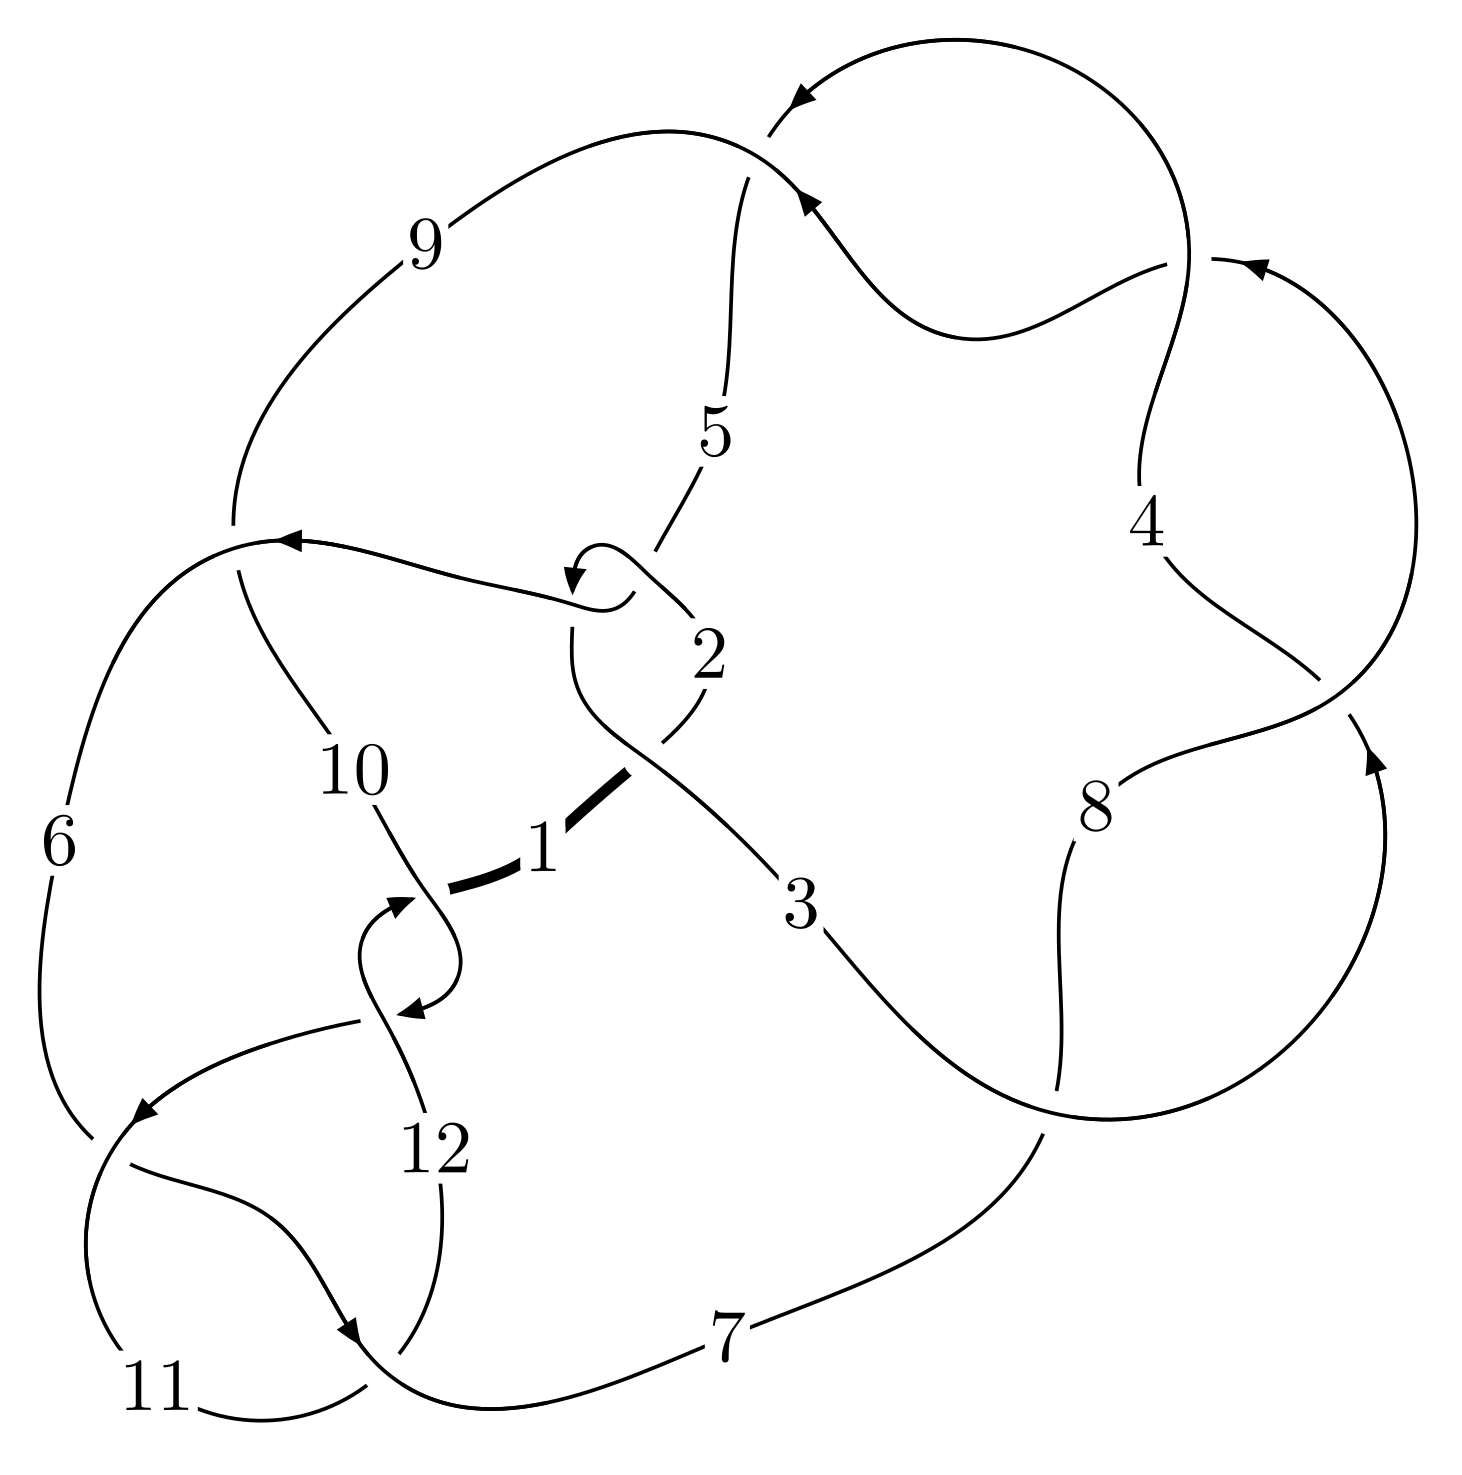
\includegraphics[width=112pt]{../../../GIT/diagram.site/Diagrams/png/2427_12n_0338.png}\\
\ \ \ A knot diagram\footnotemark}&
\allowdisplaybreaks
\textbf{Linearized knot diagam} \\
\cline{2-2}
 &
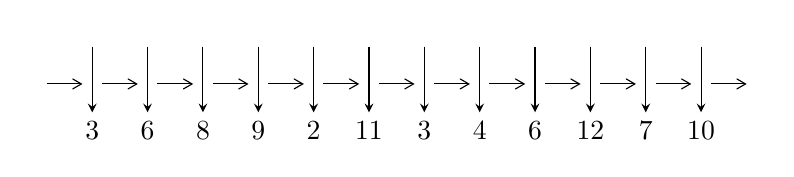
\begin{tikzpicture}[x=20pt, y=17pt]
	% nodes
	\node (C0) at (0, 0) {};
	\node (C1) at (1, 0) {};
	\node (C1U) at (1, +1) {};
	\node (C1D) at (1, -1) {3};

	\node (C2) at (2, 0) {};
	\node (C2U) at (2, +1) {};
	\node (C2D) at (2, -1) {6};

	\node (C3) at (3, 0) {};
	\node (C3U) at (3, +1) {};
	\node (C3D) at (3, -1) {8};

	\node (C4) at (4, 0) {};
	\node (C4U) at (4, +1) {};
	\node (C4D) at (4, -1) {9};

	\node (C5) at (5, 0) {};
	\node (C5U) at (5, +1) {};
	\node (C5D) at (5, -1) {2};

	\node (C6) at (6, 0) {};
	\node (C6U) at (6, +1) {};
	\node (C6D) at (6, -1) {11};

	\node (C7) at (7, 0) {};
	\node (C7U) at (7, +1) {};
	\node (C7D) at (7, -1) {3};

	\node (C8) at (8, 0) {};
	\node (C8U) at (8, +1) {};
	\node (C8D) at (8, -1) {4};

	\node (C9) at (9, 0) {};
	\node (C9U) at (9, +1) {};
	\node (C9D) at (9, -1) {6};

	\node (C10) at (10, 0) {};
	\node (C10U) at (10, +1) {};
	\node (C10D) at (10, -1) {12};

	\node (C11) at (11, 0) {};
	\node (C11U) at (11, +1) {};
	\node (C11D) at (11, -1) {7};

	\node (C12) at (12, 0) {};
	\node (C12U) at (12, +1) {};
	\node (C12D) at (12, -1) {10};
	\node (C13) at (13, 0) {};

	% arrows
	\draw[->,>={angle 60}]
	(C0) edge (C1) (C1) edge (C2) (C2) edge (C3) (C3) edge (C4) (C4) edge (C5) (C5) edge (C6) (C6) edge (C7) (C7) edge (C8) (C8) edge (C9) (C9) edge (C10) (C10) edge (C11) (C11) edge (C12) (C12) edge (C13) ;	\draw[->,>=stealth]
	(C1U) edge (C1D) (C2U) edge (C2D) (C3U) edge (C3D) (C4U) edge (C4D) (C5U) edge (C5D) (C6U) edge (C6D) (C7U) edge (C7D) (C8U) edge (C8D) (C9U) edge (C9D) (C10U) edge (C10D) (C11U) edge (C11D) (C12U) edge (C12D) ;
	\end{tikzpicture} \\
\hhline{~~} \\& 
\textbf{Solving Sequence} \\ \cline{2-2} 
 &
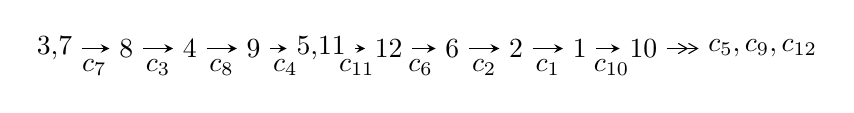
\begin{tikzpicture}[x=23pt, y=7pt]
	% node
	\node (A0) at (-1/8, 0) {3,7};
	\node (A1) at (1, 0) {8};
	\node (A2) at (2, 0) {4};
	\node (A3) at (3, 0) {9};
	\node (A4) at (65/16, 0) {5,11};
	\node (A5) at (41/8, 0) {12};
	\node (A6) at (49/8, 0) {6};
	\node (A7) at (57/8, 0) {2};
	\node (A8) at (65/8, 0) {1};
	\node (A9) at (73/8, 0) {10};
	\node (C1) at (1/2, -1) {$c_{7}$};
	\node (C2) at (3/2, -1) {$c_{3}$};
	\node (C3) at (5/2, -1) {$c_{8}$};
	\node (C4) at (7/2, -1) {$c_{4}$};
	\node (C5) at (37/8, -1) {$c_{11}$};
	\node (C6) at (45/8, -1) {$c_{6}$};
	\node (C7) at (53/8, -1) {$c_{2}$};
	\node (C8) at (61/8, -1) {$c_{1}$};
	\node (C9) at (69/8, -1) {$c_{10}$};
	\node (A10) at (11, 0) {$c_{5},c_{9},c_{12}$};

	% edge
	\draw[->,>=stealth]	
	(A0) edge (A1) (A1) edge (A2) (A2) edge (A3) (A3) edge (A4) (A4) edge (A5) (A5) edge (A6) (A6) edge (A7) (A7) edge (A8) (A8) edge (A9) ;
	\draw[->>,>={angle 60}]	
	(A9) edge (A10);
\end{tikzpicture} \\ 

\end{tabular} \\

\footnotetext{
The image of knot diagram is generated by the software ``\textbf{Draw programme}" developed by Andrew Bartholomew(\url{http://www.layer8.co.uk/maths/draw/index.htm\#Running-draw}), where we modified some parts for our purpose(\url{https://github.com/CATsTAILs/LinksPainter}).
}\phantom \\ \newline 
\centering \textbf{Ideals for irreducible components\footnotemark of $X_{\text{par}}$} 
 
\begin{align*}
I^u_{1}&=\langle 
-3004101246716 u^{20}-373089817451 u^{19}+\cdots+21082954445324 b+26346240192572,\\
\phantom{I^u_{1}}&\phantom{= \langle  }1831272589986 u^{20}+602119374746 u^{19}+\cdots+21082954445324 a-24452295430928,\\
\phantom{I^u_{1}}&\phantom{= \langle  }u^{21}+u^{20}+\cdots+8 u-8\rangle \\
I^u_{2}&=\langle 
4 a^2 u+6 a^2+b-1,\;4 a^3+4 a u-6 a-7 u+10,\;u^2-2\rangle \\
\\
I^v_{1}&=\langle 
a,\;b+v+1,\;v^3+2 v^2+v+1\rangle \\
\end{align*}
\raggedright * 3 irreducible components of $\dim_{\mathbb{C}}=0$, with total 30 representations.\\
\footnotetext{All coefficients of polynomials are rational numbers. But the coefficients are sometimes approximated in decimal forms when there is not enough margin.}
\newpage
\renewcommand{\arraystretch}{1}
\centering \section*{I. $I^u_{1}= \langle -3.00\times10^{12} u^{20}-3.73\times10^{11} u^{19}+\cdots+2.11\times10^{13} b+2.63\times10^{13},\;1.83\times10^{12} u^{20}+6.02\times10^{11} u^{19}+\cdots+2.11\times10^{13} a-2.45\times10^{13},\;u^{21}+u^{20}+\cdots+8 u-8 \rangle$}
\flushleft \textbf{(i) Arc colorings}\\
\begin{tabular}{m{7pt} m{180pt} m{7pt} m{180pt} }
\flushright $a_{3}=$&$\begin{pmatrix}0\\u\end{pmatrix}$ \\
\flushright $a_{7}=$&$\begin{pmatrix}1\\0\end{pmatrix}$ \\
\flushright $a_{8}=$&$\begin{pmatrix}1\\u^2\end{pmatrix}$ \\
\flushright $a_{4}=$&$\begin{pmatrix}- u\\- u^3+u\end{pmatrix}$ \\
\flushright $a_{9}=$&$\begin{pmatrix}- u^2+1\\- u^4+2 u^2\end{pmatrix}$ \\
\flushright $a_{5}=$&$\begin{pmatrix}u^3-2 u\\u^5-3 u^3+u\end{pmatrix}$ \\
\flushright $a_{11}=$&$\begin{pmatrix}-0.0868603 u^{20}-0.0285595 u^{19}+\cdots-0.459641 u+1.15981\\0.142490 u^{20}+0.0176963 u^{19}+\cdots+2.40462 u-1.24965\end{pmatrix}$ \\
\flushright $a_{12}=$&$\begin{pmatrix}-0.229350 u^{20}-0.0462558 u^{19}+\cdots-2.86426 u+2.40946\\0.142490 u^{20}+0.0176963 u^{19}+\cdots+2.40462 u-1.24965\end{pmatrix}$ \\
\flushright $a_{6}=$&$\begin{pmatrix}-0.138686 u^{20}+0.00718333 u^{19}+\cdots-0.505659 u+1.36119\\-0.242033 u^{20}+0.00703747 u^{19}+\cdots-5.49406 u+2.13835\end{pmatrix}$ \\
\flushright $a_{2}=$&$\begin{pmatrix}-0.128794 u^{20}+0.0122843 u^{19}+\cdots-3.05410 u+1.34108\\-0.237410 u^{20}-0.0250130 u^{19}+\cdots-2.82817 u+2.12013\end{pmatrix}$ \\
\flushright $a_{1}=$&$\begin{pmatrix}-0.128794 u^{20}+0.0122843 u^{19}+\cdots-3.05410 u+1.34108\\-0.111694 u^{20}-0.00741087 u^{19}+\cdots-0.669180 u+0.991499\end{pmatrix}$ \\
\flushright $a_{10}=$&$\begin{pmatrix}-0.121424 u^{20}-0.0196218 u^{19}+\cdots-2.92331 u+2.24622\\-0.185607 u^{20}-0.0285721 u^{19}+\cdots-2.65413 u+1.26626\end{pmatrix}$\\&\end{tabular}
\flushleft \textbf{(ii) Obstruction class $= -1$}\\~\\
\flushleft \textbf{(iii) Cusp Shapes $= \frac{29083336030791}{21082954445324} u^{20}-\frac{503291539209}{21082954445324} u^{19}+\cdots+\frac{136967234579540}{5270738611331} u-\frac{144077080803222}{5270738611331}$}\\~\\
\newpage\renewcommand{\arraystretch}{1}
\flushleft \textbf{(iv) u-Polynomials at the component}\newline \\
\begin{tabular}{m{50pt}|m{274pt}}
Crossings & \hspace{64pt}u-Polynomials at each crossing \\
\hline $$\begin{aligned}c_{1}\end{aligned}$$&$\begin{aligned}
&u^{21}+36 u^{20}+\cdots+11991 u+529
\end{aligned}$\\
\hline $$\begin{aligned}c_{2},c_{5}\end{aligned}$$&$\begin{aligned}
&u^{21}+4 u^{20}+\cdots-59 u-23
\end{aligned}$\\
\hline $$\begin{aligned}c_{3},c_{4},c_{7}\\c_{8}\end{aligned}$$&$\begin{aligned}
&u^{21}- u^{20}+\cdots+8 u+8
\end{aligned}$\\
\hline $$\begin{aligned}c_{6},c_{11}\end{aligned}$$&$\begin{aligned}
&u^{21}-2 u^{20}+\cdots+8 u^2-1
\end{aligned}$\\
\hline $$\begin{aligned}c_{9}\end{aligned}$$&$\begin{aligned}
&u^{21}+2 u^{20}+\cdots-144 u-52
\end{aligned}$\\
\hline $$\begin{aligned}c_{10},c_{12}\end{aligned}$$&$\begin{aligned}
&u^{21}+10 u^{20}+\cdots+16 u+1
\end{aligned}$\\
\hline
\end{tabular}\\~\\
\newpage\renewcommand{\arraystretch}{1}
\flushleft \textbf{(v) Riley Polynomials at the component}\newline \\
\begin{tabular}{m{50pt}|m{274pt}}
Crossings & \hspace{64pt}Riley Polynomials at each crossing \\
\hline $$\begin{aligned}c_{1}\end{aligned}$$&$\begin{aligned}
&y^{21}-92 y^{20}+\cdots+39622923 y-279841
\end{aligned}$\\
\hline $$\begin{aligned}c_{2},c_{5}\end{aligned}$$&$\begin{aligned}
&y^{21}-36 y^{20}+\cdots+11991 y-529
\end{aligned}$\\
\hline $$\begin{aligned}c_{3},c_{4},c_{7}\\c_{8}\end{aligned}$$&$\begin{aligned}
&y^{21}-35 y^{20}+\cdots+320 y-64
\end{aligned}$\\
\hline $$\begin{aligned}c_{6},c_{11}\end{aligned}$$&$\begin{aligned}
&y^{21}-10 y^{20}+\cdots+16 y-1
\end{aligned}$\\
\hline $$\begin{aligned}c_{9}\end{aligned}$$&$\begin{aligned}
&y^{21}-66 y^{20}+\cdots+76376 y-2704
\end{aligned}$\\
\hline $$\begin{aligned}c_{10},c_{12}\end{aligned}$$&$\begin{aligned}
&y^{21}+6 y^{20}+\cdots+96 y-1
\end{aligned}$\\
\hline
\end{tabular}\\~\\
\newpage\flushleft \textbf{(vi) Complex Volumes and Cusp Shapes}
$$\begin{array}{c|c|c}  
\text{Solutions to }I^u_{1}& \I (\text{vol} + \sqrt{-1}CS) & \text{Cusp shape}\\
 \hline 
\begin{aligned}
u &= -0.901926 + 0.051407 I \\
a &= \phantom{-}1.58428 + 0.44230 I \\
b &= \phantom{-}0.929270 - 0.621178 I\end{aligned}
 & -0.70179 + 4.44296 I & -15.1059 - 6.6514 I \\ \hline\begin{aligned}
u &= -0.901926 - 0.051407 I \\
a &= \phantom{-}1.58428 - 0.44230 I \\
b &= \phantom{-}0.929270 + 0.621178 I\end{aligned}
 & -0.70179 - 4.44296 I & -15.1059 + 6.6514 I \\ \hline\begin{aligned}
u &= -0.487980 + 0.535998 I \\
a &= -1.29130 - 1.86784 I \\
b &= -0.972602 + 0.217979 I\end{aligned}
 & -3.41098 + 0.72478 I & -18.1754 - 4.1507 I \\ \hline\begin{aligned}
u &= -0.487980 - 0.535998 I \\
a &= -1.29130 + 1.86784 I \\
b &= -0.972602 - 0.217979 I\end{aligned}
 & -3.41098 - 0.72478 I & -18.1754 + 4.1507 I \\ \hline\begin{aligned}
u &= \phantom{-}0.667009 + 0.250056 I \\
a &= \phantom{-}0.473812 - 0.352817 I \\
b &= \phantom{-}0.746002 - 0.517025 I\end{aligned}
 & -0.131566 + 0.215455 I & -13.55030 + 1.35945 I \\ \hline\begin{aligned}
u &= \phantom{-}0.667009 - 0.250056 I \\
a &= \phantom{-}0.473812 + 0.352817 I \\
b &= \phantom{-}0.746002 + 0.517025 I\end{aligned}
 & -0.131566 - 0.215455 I & -13.55030 - 1.35945 I \\ \hline\begin{aligned}
u &= -1.336150 + 0.286473 I \\
a &= -0.480443 - 0.210578 I \\
b &= \phantom{-}0.219656 + 0.684964 I\end{aligned}
 & -6.45258 + 0.58096 I & -15.0688 - 0.0562 I \\ \hline\begin{aligned}
u &= -1.336150 - 0.286473 I \\
a &= -0.480443 + 0.210578 I \\
b &= \phantom{-}0.219656 - 0.684964 I\end{aligned}
 & -6.45258 - 0.58096 I & -15.0688 + 0.0562 I \\ \hline\begin{aligned}
u &= -1.46037\phantom{ +0.000000I} \\
a &= -1.04497\phantom{ +0.000000I} \\
b &= -0.429188\phantom{ +0.000000I}\end{aligned}
 & -6.73694\phantom{ +0.000000I} & -12.3530\phantom{ +0.000000I} \\ \hline\begin{aligned}
u &= \phantom{-}1.37773 + 0.63713 I \\
a &= \phantom{-}1.24070 - 1.07467 I \\
b &= \phantom{-}1.177670 + 0.522691 I\end{aligned}
 & -9.24475 - 5.31786 I & -17.8058 + 4.0813 I\\
 \hline 
 \end{array}$$\newpage$$\begin{array}{c|c|c}  
\text{Solutions to }I^u_{1}& \I (\text{vol} + \sqrt{-1}CS) & \text{Cusp shape}\\
 \hline 
\begin{aligned}
u &= \phantom{-}1.37773 - 0.63713 I \\
a &= \phantom{-}1.24070 + 1.07467 I \\
b &= \phantom{-}1.177670 - 0.522691 I\end{aligned}
 & -9.24475 + 5.31786 I & -17.8058 - 4.0813 I \\ \hline\begin{aligned}
u &= \phantom{-}0.007014 + 0.428132 I \\
a &= \phantom{-}0.157773 + 1.318050 I \\
b &= -0.876187 - 0.694943 I\end{aligned}
 & \phantom{-}2.12758 - 2.67655 I & -5.20055 + 2.49560 I \\ \hline\begin{aligned}
u &= \phantom{-}0.007014 - 0.428132 I \\
a &= \phantom{-}0.157773 - 1.318050 I \\
b &= -0.876187 + 0.694943 I\end{aligned}
 & \phantom{-}2.12758 + 2.67655 I & -5.20055 - 2.49560 I \\ \hline\begin{aligned}
u &= \phantom{-}0.380480\phantom{ +0.000000I} \\
a &= \phantom{-}0.651164\phantom{ +0.000000I} \\
b &= \phantom{-}0.349133\phantom{ +0.000000I}\end{aligned}
 & -0.576083\phantom{ +0.000000I} & -17.0820\phantom{ +0.000000I} \\ \hline\begin{aligned}
u &= \phantom{-}1.73579 + 0.22895 I \\
a &= -1.43373 + 0.00630 I \\
b &= -1.176150 + 0.419094 I\end{aligned}
 & -10.01720 + 3.13008 I & -18.2978 - 3.1992 I \\ \hline\begin{aligned}
u &= \phantom{-}1.73579 - 0.22895 I \\
a &= -1.43373 - 0.00630 I \\
b &= -1.176150 - 0.419094 I\end{aligned}
 & -10.01720 - 3.13008 I & -18.2978 + 3.1992 I \\ \hline\begin{aligned}
u &= \phantom{-}1.90238 + 0.14731 I \\
a &= -0.0278466 + 0.0602262 I \\
b &= -0.516255 + 1.062480 I\end{aligned}
 & -18.6129 - 3.3460 I & -15.4445 + 0.4593 I \\ \hline\begin{aligned}
u &= \phantom{-}1.90238 - 0.14731 I \\
a &= -0.0278466 - 0.0602262 I \\
b &= -0.516255 - 1.062480 I\end{aligned}
 & -18.6129 + 3.3460 I & -15.4445 - 0.4593 I \\ \hline\begin{aligned}
u &= -1.89336 + 0.24852 I \\
a &= -1.27473 - 0.71223 I \\
b &= -1.194710 + 0.746952 I\end{aligned}
 & \phantom{-}18.7399 + 9.8858 I & -17.0280 - 4.3210 I \\ \hline\begin{aligned}
u &= -1.89336 - 0.24852 I \\
a &= -1.27473 + 0.71223 I \\
b &= -1.194710 - 0.746952 I\end{aligned}
 & \phantom{-}18.7399 - 9.8858 I & -17.0280 + 4.3210 I\\
 \hline 
 \end{array}$$\newpage$$\begin{array}{c|c|c}  
\text{Solutions to }I^u_{1}& \I (\text{vol} + \sqrt{-1}CS) & \text{Cusp shape}\\
 \hline 
\begin{aligned}
u &= -2.06112\phantom{ +0.000000I} \\
a &= \phantom{-}1.49678\phantom{ +0.000000I} \\
b &= \phantom{-}1.40668\phantom{ +0.000000I}\end{aligned}
 & \phantom{-}13.3737\phantom{ +0.000000I} & -19.2100\phantom{ +0.000000I}\\
 \hline 
 \end{array}$$\newpage\newpage\renewcommand{\arraystretch}{1}
\centering \section*{II. $I^u_{2}= \langle 4 a^2 u+6 a^2+b-1,\;4 a^3+4 a u-6 a-7 u+10,\;u^2-2 \rangle$}
\flushleft \textbf{(i) Arc colorings}\\
\begin{tabular}{m{7pt} m{180pt} m{7pt} m{180pt} }
\flushright $a_{3}=$&$\begin{pmatrix}0\\u\end{pmatrix}$ \\
\flushright $a_{7}=$&$\begin{pmatrix}1\\0\end{pmatrix}$ \\
\flushright $a_{8}=$&$\begin{pmatrix}1\\2\end{pmatrix}$ \\
\flushright $a_{4}=$&$\begin{pmatrix}- u\\- u\end{pmatrix}$ \\
\flushright $a_{9}=$&$\begin{pmatrix}-1\\0\end{pmatrix}$ \\
\flushright $a_{5}=$&$\begin{pmatrix}0\\- u\end{pmatrix}$ \\
\flushright $a_{11}=$&$\begin{pmatrix}a\\-4 a^2 u-6 a^2+1\end{pmatrix}$ \\
\flushright $a_{12}=$&$\begin{pmatrix}4 a^2 u+6 a^2+a-1\\-4 a^2 u-6 a^2+1\end{pmatrix}$ \\
\flushright $a_{6}=$&$\begin{pmatrix}\frac{1}{2} u\\4 a^2 u+6 a^2+a u+2 a-1\end{pmatrix}$ \\
\flushright $a_{2}=$&$\begin{pmatrix}\frac{1}{2} u\\4 a^2 u+6 a^2+a u+2 a+u-1\end{pmatrix}$ \\
\flushright $a_{1}=$&$\begin{pmatrix}\frac{1}{2} u\\4 a^2 u+6 a^2+a u+2 a-1\end{pmatrix}$ \\
\flushright $a_{10}=$&$\begin{pmatrix}-3 a^2 u-4 a^2- a u- a+\frac{1}{2} u-1\\a u+2 a+1\end{pmatrix}$\\&\end{tabular}
\flushleft \textbf{(ii) Obstruction class $= 1$}\\~\\
\flushleft \textbf{(iii) Cusp Shapes $= -16 a^2 u-24 a^2-16$}\\~\\
\newpage\renewcommand{\arraystretch}{1}
\flushleft \textbf{(iv) u-Polynomials at the component}\newline \\
\begin{tabular}{m{50pt}|m{274pt}}
Crossings & \hspace{64pt}u-Polynomials at each crossing \\
\hline $$\begin{aligned}c_{1},c_{5}\end{aligned}$$&$\begin{aligned}
&(u-1)^6
\end{aligned}$\\
\hline $$\begin{aligned}c_{2}\end{aligned}$$&$\begin{aligned}
&(u+1)^6
\end{aligned}$\\
\hline $$\begin{aligned}c_{3},c_{4},c_{7}\\c_{8}\end{aligned}$$&$\begin{aligned}
&(u^2-2)^3
\end{aligned}$\\
\hline $$\begin{aligned}c_{6}\end{aligned}$$&$\begin{aligned}
&(u^3- u^2+1)^2
\end{aligned}$\\
\hline $$\begin{aligned}c_{9},c_{10}\end{aligned}$$&$\begin{aligned}
&(u^3- u^2+2 u-1)^2
\end{aligned}$\\
\hline $$\begin{aligned}c_{11}\end{aligned}$$&$\begin{aligned}
&(u^3+u^2-1)^2
\end{aligned}$\\
\hline $$\begin{aligned}c_{12}\end{aligned}$$&$\begin{aligned}
&(u^3+u^2+2 u+1)^2
\end{aligned}$\\
\hline
\end{tabular}\\~\\
\newpage\renewcommand{\arraystretch}{1}
\flushleft \textbf{(v) Riley Polynomials at the component}\newline \\
\begin{tabular}{m{50pt}|m{274pt}}
Crossings & \hspace{64pt}Riley Polynomials at each crossing \\
\hline $$\begin{aligned}c_{1},c_{2},c_{5}\end{aligned}$$&$\begin{aligned}
&(y-1)^6
\end{aligned}$\\
\hline $$\begin{aligned}c_{3},c_{4},c_{7}\\c_{8}\end{aligned}$$&$\begin{aligned}
&(y-2)^6
\end{aligned}$\\
\hline $$\begin{aligned}c_{6},c_{11}\end{aligned}$$&$\begin{aligned}
&(y^3- y^2+2 y-1)^2
\end{aligned}$\\
\hline $$\begin{aligned}c_{9},c_{10},c_{12}\end{aligned}$$&$\begin{aligned}
&(y^3+3 y^2+2 y-1)^2
\end{aligned}$\\
\hline
\end{tabular}\\~\\
\newpage\flushleft \textbf{(vi) Complex Volumes and Cusp Shapes}
$$\begin{array}{c|c|c}  
\text{Solutions to }I^u_{2}& \I (\text{vol} + \sqrt{-1}CS) & \text{Cusp shape}\\
 \hline 
\begin{aligned}
u &= \phantom{-}1.41421\phantom{ +0.000000I} \\
a &= -0.388001\phantom{ +0.000000I} \\
b &= -0.754878\phantom{ +0.000000I}\end{aligned}
 & -7.69319\phantom{ +0.000000I} & -23.0200\phantom{ +0.000000I} \\ \hline\begin{aligned}
u &= \phantom{-}1.41421\phantom{ +0.000000I} \\
a &= \phantom{-}0.194000 + 0.164688 I \\
b &= \phantom{-}0.877439 - 0.744862 I\end{aligned}
 & -3.55561 + 2.82812 I & -16.4902 - 2.9794 I \\ \hline\begin{aligned}
u &= \phantom{-}1.41421\phantom{ +0.000000I} \\
a &= \phantom{-}0.194000 - 0.164688 I \\
b &= \phantom{-}0.877439 + 0.744862 I\end{aligned}
 & -3.55561 - 2.82812 I & -16.4902 + 2.9794 I \\ \hline\begin{aligned}
u &= -1.41421\phantom{ +0.000000I} \\
a &= \phantom{-}1.13072 + 0.95987 I \\
b &= \phantom{-}0.877439 - 0.744862 I\end{aligned}
 & -3.55561 + 2.82812 I & -16.4902 - 2.9794 I \\ \hline\begin{aligned}
u &= -1.41421\phantom{ +0.000000I} \\
a &= \phantom{-}1.13072 - 0.95987 I \\
b &= \phantom{-}0.877439 + 0.744862 I\end{aligned}
 & -3.55561 - 2.82812 I & -16.4902 + 2.9794 I \\ \hline\begin{aligned}
u &= -1.41421\phantom{ +0.000000I} \\
a &= -2.26144\phantom{ +0.000000I} \\
b &= -0.754878\phantom{ +0.000000I}\end{aligned}
 & -7.69319\phantom{ +0.000000I} & -23.0200\phantom{ +0.000000I}\\
 \hline 
 \end{array}$$\newpage\newpage\renewcommand{\arraystretch}{1}
\centering \section*{III. $I^v_{1}= \langle a,\;b+v+1,\;v^3+2 v^2+v+1 \rangle$}
\flushleft \textbf{(i) Arc colorings}\\
\begin{tabular}{m{7pt} m{180pt} m{7pt} m{180pt} }
\flushright $a_{3}=$&$\begin{pmatrix}v\\0\end{pmatrix}$ \\
\flushright $a_{7}=$&$\begin{pmatrix}1\\0\end{pmatrix}$ \\
\flushright $a_{8}=$&$\begin{pmatrix}1\\0\end{pmatrix}$ \\
\flushright $a_{4}=$&$\begin{pmatrix}v\\0\end{pmatrix}$ \\
\flushright $a_{9}=$&$\begin{pmatrix}1\\0\end{pmatrix}$ \\
\flushright $a_{5}=$&$\begin{pmatrix}v\\0\end{pmatrix}$ \\
\flushright $a_{11}=$&$\begin{pmatrix}0\\- v-1\end{pmatrix}$ \\
\flushright $a_{12}=$&$\begin{pmatrix}v+1\\- v-1\end{pmatrix}$ \\
\flushright $a_{6}=$&$\begin{pmatrix}1\\- v^2-2 v-1\end{pmatrix}$ \\
\flushright $a_{2}=$&$\begin{pmatrix}v-1\\v^2+2 v+1\end{pmatrix}$ \\
\flushright $a_{1}=$&$\begin{pmatrix}-1\\v^2+2 v+1\end{pmatrix}$ \\
\flushright $a_{10}=$&$\begin{pmatrix}- v^2-2 v\\v^2+v-1\end{pmatrix}$\\&\end{tabular}
\flushleft \textbf{(ii) Obstruction class $= 1$}\\~\\
\flushleft \textbf{(iii) Cusp Shapes $= 4 v^2+6 v-14$}\\~\\
\newpage\renewcommand{\arraystretch}{1}
\flushleft \textbf{(iv) u-Polynomials at the component}\newline \\
\begin{tabular}{m{50pt}|m{274pt}}
Crossings & \hspace{64pt}u-Polynomials at each crossing \\
\hline $$\begin{aligned}c_{1},c_{2}\end{aligned}$$&$\begin{aligned}
&(u-1)^3
\end{aligned}$\\
\hline $$\begin{aligned}c_{3},c_{4},c_{7}\\c_{8}\end{aligned}$$&$\begin{aligned}
&u^3
\end{aligned}$\\
\hline $$\begin{aligned}c_{5}\end{aligned}$$&$\begin{aligned}
&(u+1)^3
\end{aligned}$\\
\hline $$\begin{aligned}c_{6}\end{aligned}$$&$\begin{aligned}
&u^3+u^2-1
\end{aligned}$\\
\hline $$\begin{aligned}c_{9},c_{12}\end{aligned}$$&$\begin{aligned}
&u^3+u^2+2 u+1
\end{aligned}$\\
\hline $$\begin{aligned}c_{10}\end{aligned}$$&$\begin{aligned}
&u^3- u^2+2 u-1
\end{aligned}$\\
\hline $$\begin{aligned}c_{11}\end{aligned}$$&$\begin{aligned}
&u^3- u^2+1
\end{aligned}$\\
\hline
\end{tabular}\\~\\
\newpage\renewcommand{\arraystretch}{1}
\flushleft \textbf{(v) Riley Polynomials at the component}\newline \\
\begin{tabular}{m{50pt}|m{274pt}}
Crossings & \hspace{64pt}Riley Polynomials at each crossing \\
\hline $$\begin{aligned}c_{1},c_{2},c_{5}\end{aligned}$$&$\begin{aligned}
&(y-1)^3
\end{aligned}$\\
\hline $$\begin{aligned}c_{3},c_{4},c_{7}\\c_{8}\end{aligned}$$&$\begin{aligned}
&y^3
\end{aligned}$\\
\hline $$\begin{aligned}c_{6},c_{11}\end{aligned}$$&$\begin{aligned}
&y^3- y^2+2 y-1
\end{aligned}$\\
\hline $$\begin{aligned}c_{9},c_{10},c_{12}\end{aligned}$$&$\begin{aligned}
&y^3+3 y^2+2 y-1
\end{aligned}$\\
\hline
\end{tabular}\\~\\
\newpage\flushleft \textbf{(vi) Complex Volumes and Cusp Shapes}
$$\begin{array}{c|c|c}  
\text{Solutions to }I^v_{1}& \I (\text{vol} + \sqrt{-1}CS) & \text{Cusp shape}\\
 \hline 
\begin{aligned}
v &= -0.122561 + 0.744862 I \\
a &= \phantom{-0.000000 } 0 \\
b &= -0.877439 - 0.744862 I\end{aligned}
 & \phantom{-}1.37919 - 2.82812 I & -16.8946 + 3.7388 I \\ \hline\begin{aligned}
v &= -0.122561 - 0.744862 I \\
a &= \phantom{-0.000000 } 0 \\
b &= -0.877439 + 0.744862 I\end{aligned}
 & \phantom{-}1.37919 + 2.82812 I & -16.8946 - 3.7388 I \\ \hline\begin{aligned}
v &= -1.75488\phantom{ +0.000000I} \\
a &= \phantom{-0.000000 } 0 \\
b &= \phantom{-}0.754878\phantom{ +0.000000I}\end{aligned}
 & -2.75839\phantom{ +0.000000I} & -12.2110\phantom{ +0.000000I}\\
 \hline 
 \end{array}$$\newpage
\newpage\renewcommand{\arraystretch}{1}
\centering \section*{ IV. u-Polynomials}
\begin{tabular}{m{50pt}|m{274pt}}
Crossings & \hspace{64pt}u-Polynomials at each crossing \\
\hline $$\begin{aligned}c_{1}\end{aligned}$$&$\begin{aligned}
&((u-1)^9)(u^{21}+36 u^{20}+\cdots+11991 u+529)
\end{aligned}$\\
\hline $$\begin{aligned}c_{2}\end{aligned}$$&$\begin{aligned}
&((u-1)^3)(u+1)^6(u^{21}+4 u^{20}+\cdots-59 u-23)
\end{aligned}$\\
\hline $$\begin{aligned}c_{3},c_{4},c_{7}\\c_{8}\end{aligned}$$&$\begin{aligned}
&u^3(u^2-2)^3(u^{21}- u^{20}+\cdots+8 u+8)
\end{aligned}$\\
\hline $$\begin{aligned}c_{5}\end{aligned}$$&$\begin{aligned}
&((u-1)^6)(u+1)^3(u^{21}+4 u^{20}+\cdots-59 u-23)
\end{aligned}$\\
\hline $$\begin{aligned}c_{6}\end{aligned}$$&$\begin{aligned}
&((u^3- u^2+1)^2)(u^3+u^2-1)(u^{21}-2 u^{20}+\cdots+8 u^2-1)
\end{aligned}$\\
\hline $$\begin{aligned}c_{9}\end{aligned}$$&$\begin{aligned}
&((u^3- u^2+2 u-1)^2)(u^3+u^2+2 u+1)(u^{21}+2 u^{20}+\cdots-144 u-52)
\end{aligned}$\\
\hline $$\begin{aligned}c_{10}\end{aligned}$$&$\begin{aligned}
&((u^3- u^2+2 u-1)^3)(u^{21}+10 u^{20}+\cdots+16 u+1)
\end{aligned}$\\
\hline $$\begin{aligned}c_{11}\end{aligned}$$&$\begin{aligned}
&(u^3- u^2+1)(u^3+u^2-1)^2(u^{21}-2 u^{20}+\cdots+8 u^2-1)
\end{aligned}$\\
\hline $$\begin{aligned}c_{12}\end{aligned}$$&$\begin{aligned}
&((u^3+u^2+2 u+1)^3)(u^{21}+10 u^{20}+\cdots+16 u+1)
\end{aligned}$\\
\hline
\end{tabular}\newpage\renewcommand{\arraystretch}{1}
\centering \section*{ V. Riley Polynomials}
\begin{tabular}{m{50pt}|m{274pt}}
Crossings & \hspace{64pt}Riley Polynomials at each crossing \\
\hline $$\begin{aligned}c_{1}\end{aligned}$$&$\begin{aligned}
&((y-1)^9)(y^{21}-92 y^{20}+\cdots+3.96229\times10^{7} y-279841)
\end{aligned}$\\
\hline $$\begin{aligned}c_{2},c_{5}\end{aligned}$$&$\begin{aligned}
&((y-1)^9)(y^{21}-36 y^{20}+\cdots+11991 y-529)
\end{aligned}$\\
\hline $$\begin{aligned}c_{3},c_{4},c_{7}\\c_{8}\end{aligned}$$&$\begin{aligned}
&y^3(y-2)^6(y^{21}-35 y^{20}+\cdots+320 y-64)
\end{aligned}$\\
\hline $$\begin{aligned}c_{6},c_{11}\end{aligned}$$&$\begin{aligned}
&((y^3- y^2+2 y-1)^3)(y^{21}-10 y^{20}+\cdots+16 y-1)
\end{aligned}$\\
\hline $$\begin{aligned}c_{9}\end{aligned}$$&$\begin{aligned}
&((y^3+3 y^2+2 y-1)^3)(y^{21}-66 y^{20}+\cdots+76376 y-2704)
\end{aligned}$\\
\hline $$\begin{aligned}c_{10},c_{12}\end{aligned}$$&$\begin{aligned}
&((y^3+3 y^2+2 y-1)^3)(y^{21}+6 y^{20}+\cdots+96 y-1)
\end{aligned}$\\
\hline
\end{tabular}
\vskip 2pc
\end{document}